\chapter{Power \& Propulsion}
\setlength{\parindent}{15pt}
\label{ch:powe_prop}

This chapter is dedicated to the design process of both the propulsion unit and the power subsystem. In \autoref{sec:DAPNP}, the design approach is discussed, followed, in \autoref{sec:AssuPNP}, by the used assumptions. In \autoref{sec:AnalPNP}, the complete analysis is documented and the result of the design process is discussed. Finally, in \autoref{sec:VNVPNP} the validation \& verification process is described.

\section{Design Approach}
\label{sec:DAPNP}
% include WFD

\begin{figure}[H]
    \centering
    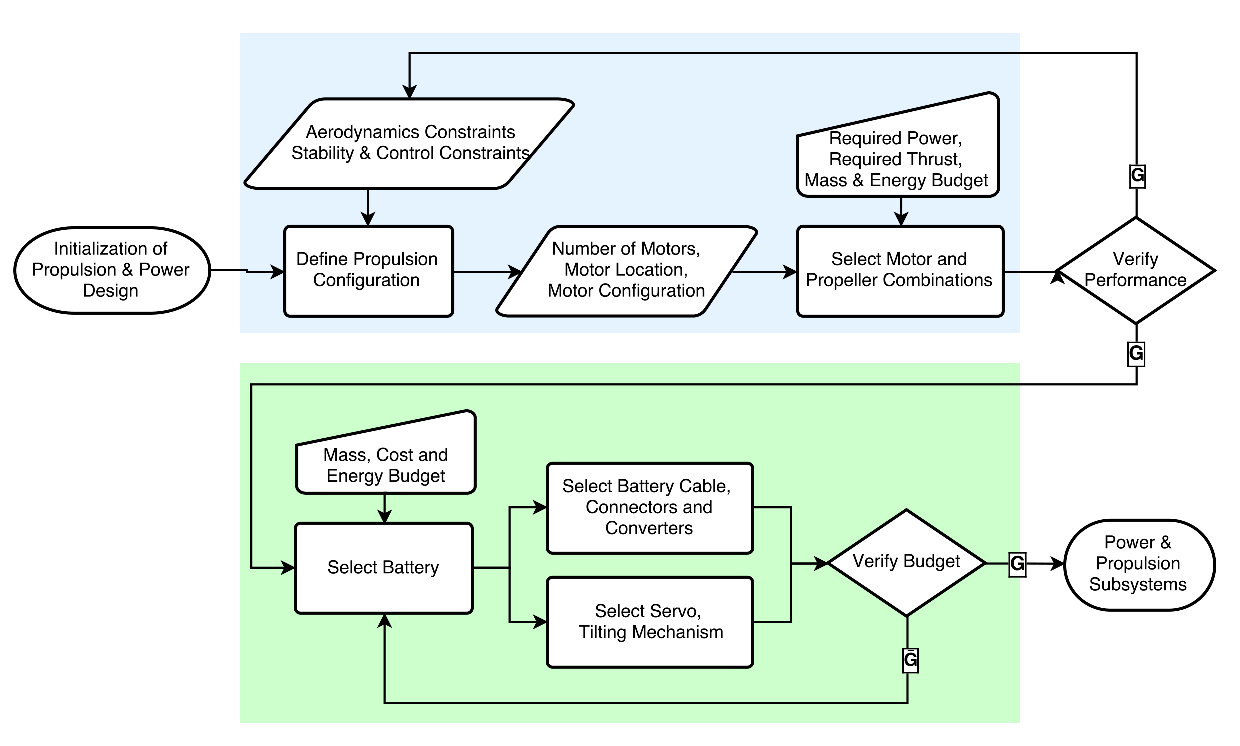
\includegraphics[width=1.0\textwidth]{PowerPropulsion/Figures/pnpwfd.pdf}
    \caption{Work Flow Diagram for Power \& Propulsion Design}
    \label{fig:wfdpnp}
\end{figure}

\autoref{fig:wfdpnp} shows the work flow diagram for the power \& propulsion design process. It includes the systematic approach and selection of the motor with propellers and power source with power distribution system based on a series of calculations. The upper blue block indicates the design process of a propulsion unit. With aerodynamics and stability \& control constraints, a series of propulsion configurations can be defined. The number of motors, motor location and motor configuration can be obtained as an output, which is used as an input for selecting a motor and propeller combination. Along with the input parameters, performance parameters such as required power, required thrust and mass \& energy budget are considered. A verification loop is performed afterwards to check if a chosen motor and propeller combination as well as a configuration is feasible based on other departments' judgements. For example, a certain combination and a configuration are passed to the stability \& control department to determine effects of the configuration. If it creates conflicts with a certain department and budgets, the department can provide the power \& propulsion group with suggestions such that a new propulsion configuration can be generated. If it is deemed feasible, the combination and configuration can be processed and relevant information is used for a battery selection process.
The lower green block indicates the design process of a power unit. Motor specifications such as power, voltage and current are used as an input for a battery selection process. The energy budget of other systems is taken into account, as the battery has to provide enough power for them. After a battery is chosen, battery-related components such as battery cables, connectors and converters are chosen based on battery specifications. Servos and tilting mechanism are selected simultaneously, as it is independent to a battery selection process. Budgets are verified to see if the chosen power unit meets budgets and requirements. After the verification loop, a complete power \& propulsion subsystem is obtained. %%%%written by Bryan @1500 21/06%%%%

%the design steps taken in the process of designing a propulsion and power system that meets the prior set requirements. This also explains the subdivision of this section into a motor and propeller part (propulsion) and an energy source subsection (power).

%The design process starts with the propulsion unit designed, after that the power unit is designed. This approach is chosen since it is more convenient to first select the right motors and afterwards come up with a corresponding battery unit. The first design block, indicated with a blue shade in \autoref{fig:wfdpnp}, covers the design approach of the propulsion unit: the motor with propellers. 

\subsection{Propulsion Unit Design Approach}
The first step in the propulsion unit design block is defining a propulsion configuration, which consists of the number of motors and their mounting location. A motor quantity analysis from three to five motors is carried out and different motor mounting systems are assessed. As the number of motors and corresponding location are chosen, off-the-shelf motors are selected. Requirement SYS-VS-3 states that the UAV shall have electrical propulsion. Although the propulsion type is constrained to be electric, a motor type still has to be determined. Two choices for a motor type are brushed and brushless. Advantages and disadvantages of each motor type are used to perform a qualitative analysis for choosing a certain motor type.

%The first step in that design block is the defining of the propulsion configuration; this means determining the number of motors and their mounting location. An analysis was done for a number of motors ranging from three to five. Also different locations were analysed, such as wing and body mounted. After the determination of the number of motors with their corresponding location, the kind of motor was chosen. Requirement SYS-VS-3 states that the UAV shall have electrical propulsion. Although propulsion type was constrained, motor type still had to be decided on; a choice had to be made between brushed and brushless motors. This was done by comparing the advantages and disadvantages of both motor types in a qualitative way.

% location of the motors on the bar (length of the bar analysis!)

%%Explain what needs to be why analysed! 
As the number of motors, motor type and location are determined, propellers can be selected. Finding a right motor and propeller combination requires a trial and error process and iterations, since a powerful motor with an arbitrary propeller does not necessarily meet desired performance requirements for VTOL and horizontal flight. Motor and propeller specifications are taken from a Hacker data set\cite{hackerdata}. \\


%At this stage, the motor type and location is constrained. For the propulsion unit design, the following approach was applied. The difficulty is to find the right motor-propeller combination, since the combination of both determines the net performance. The approach is based on 'playing around' with the different variables and try different motor-propeller combinations from the Hacker data set.


\noindent \textbf{Step 1:} The high-velocity requirement SYS-PF-1.2 is a driving requirement. The most important design aspect to attain the high velocity of 200 km/h is the propeller design. Generally, a high-pitched propeller is required for high velocity.\\

%which means we first need to ensure this performance characteristics is met. The most important design aspect to attain this 200 km/h is the propeller design; a high pitched propeller is required. \\

\nomenclature[A]{STC}{Static Thrust Calculator}

\noindent \textbf{Step 2:} After constraining the aft-propeller pitch, a propeller diameter and aft motors can be chosen. Since both the propeller diameter in combination with the after motors need to be determined, one way approach cannot be applied. There are more design parameters than the number of design constraints. An iterative approach with an use of a Static Thrust Calculator (STC) is used to find a right combination of a propeller diameter and aft motors. The team had consulted ATMOS and received advice that motors from Hacker-motors could be considered as Hacker-motors is a prominent motor manufacturer specialised in brushless motors. After a series of iterations, the right aft motor-propeller combination is found.

%After having constrained the aft propeller pitch, the propeller diameter and the aft motor could be found. Since both the propeller diameter in combination with the aft motor (with corresponding specifications) needs to be found, there are more design parameters than strains; the problem is undetermined. By means of an iterative approach and the use of a Static Thrust Calculator (STC), the right combination was found. In recommendation of ATMOS, there was chosen to limit the motor selection to the data set of Hacker-motors, a prominent German brushless-motor manufacturer. After sufficient iterations, the right aft motor-propeller combination was found.

\nomenclature[A]{PDC}{Python Drag Calculator}

For this step, a required thrust value is an input. The motors should provide sufficient thrust to overcome drag at the maximum velocity, which results in the highest drag. During the horizontal flight phase, only aft motors are operational, while the propellers on the front motors are folded in a feathering mode to minimise drag. To calculate the required thrust and power for maximum velocity cruise flight, a Python Drag Calculator (PDC) tool is used.\\ %%%% Rewritten by Bryan, stopping at 2106 to do power section and diagrams %%%%%

%In the process step 2, a required thrust is needed as input; the motor should provide sufficient thrust to overcome drag at maximum velocity, the case of highest drag. For later explained reasons, during the horizontal flight phase only the aft motors are operative; they deliver thrust while the propellers on the front motor are folded (feathering mode). To calculate the required thrust and power for maximum velocity cruise flight, a Python Drag Calculator tool was used. \\

\noindent \textbf{Step 3:} After constraining the complete aft motor-propeller combination, the VTOL performance is analysed. Since the aft motor is optimised for horizontal flight, its performance is relatively poor in VTOL. Knowing VTOL capabilities of the aft motor allows the required front motor VTOL performance to be computed. This front motor-propeller combination is to be optimised for VTOL; it means that a different motor category is considered. The required forward performance parameters such as required thrust are found by using a Python VTOL Thrust Calculator. By means of trial and error along with an iterative approach, a suitable front motor-propeller combination is selected.

\subsection{Power Subsystem Design Approach}
The power subsystem requires motor specifications as well as energy budgets of other subsystems. Unlike the propulsion subsystem design approach, the power subsystem design approach does not require intensive iterative processes. The battery is primarily sized based on extreme flight scenarios and essential flight phases, which are shown in the following list.

\begin{itemize}
    \item Extreme flight scenarios
    \begin{itemize}
        \item Max.speed horizontal flight
        \item Max.range horizontal flight
        \item Max.endurance horizontal flight    
    \end{itemize}
    \item Essential flight phases
    \begin{enumerate}
        \item VTOL
        \item Hovering
    \end{enumerate}
\end{itemize}

The other subsystems such as avionics and payload draw power from the battery, and the battery sizing increases further based on their energy budget.

As flight phases and other subsystems are considered for the battery sizing, the method for calculating a required battery capacity needs to defined. The PDC determines a required battery capacity of extreme flight conditions by calculating the required power per scenario then coveting it to the battery capacity in [mAh]. The most extreme flight scenario is identified as well as two essential flight phases and power usage of other subsystems for the final battery sizing.

\section{Assumptions}
\label{sec:AssuPNP}
This section contains the made assumptions in the design process of both the propulsion and the power subsystem and the effect on them. 

\paragraph{General simplifications:}
\begin{itemize}
    \item Power used by servos are minimal, thus negligible.
    \item The relation between battery capacity and range is linear, due to the fact that power consumed during horizontal flight is approximately constant.
\end{itemize}

\paragraph{Hardware related:} 
\begin{itemize}
    \item Chosen servos are waterproof, by means of an internal waterproof construction or an external protective casing.
    \item Propellers do not have to be designed completely, as only off-the-shelf components components will be considered.
    \item Motors are chosen from off-the-shelf motors, from a data sheet of the manufacturer Hacker-motors.
    \item Back propellers can be used as pusher propellers, regardless of availability of pusher propellers for right dimensions.
\end{itemize}

\paragraph{Efficiency related:} 
\begin{itemize}
    \item Front motor efficiency is 90\%.
    \item Aft motor efficiency is 95\%
    \item Calculations are done for optimally-performing propellers.
\end{itemize}

\noindent Motor efficiencies were not provided by the manufacturer. By means of a efficiency calculator, the order of magnitude of the motor was estimated and included as an assumption. Because no exotic propeller configurations (such as propeller wash phenomena due to aligned propellers) are applied, and the propeller used for this UAV is an of-the-shelf component, no further research was done for propeller efficiency.  

\paragraph{Flight condition related:}
\begin{itemize}
    \item Operational temperature is 15 degrees Celsius. 
    \item Air density at operational altitude is equal to sea level density, which is 1.225 kg/$m^3$
\end{itemize}


\section{Analysis} %% MUST BE REVISED !!!!!
\label{sec:AnalPNP}
This section contains the analysis of a motor configuration and a motor type. Then tools used are elaborated; the required inputs and outputs, theoretical background and equations are stated.

\subsection{Motor and Propellers}
\label{sec:MP}

\paragraph{Motor configuration:} Different number of motors with corresponding locations are analysed. The different locations are leading-edge mounted, wing-mounted quadcopter setting and body-mounted. The number of motors varies from three to five. The analysed configurations can bee seen in \autoref{fig:motorconfig}.

\begin{figure}[H]
    \centering
    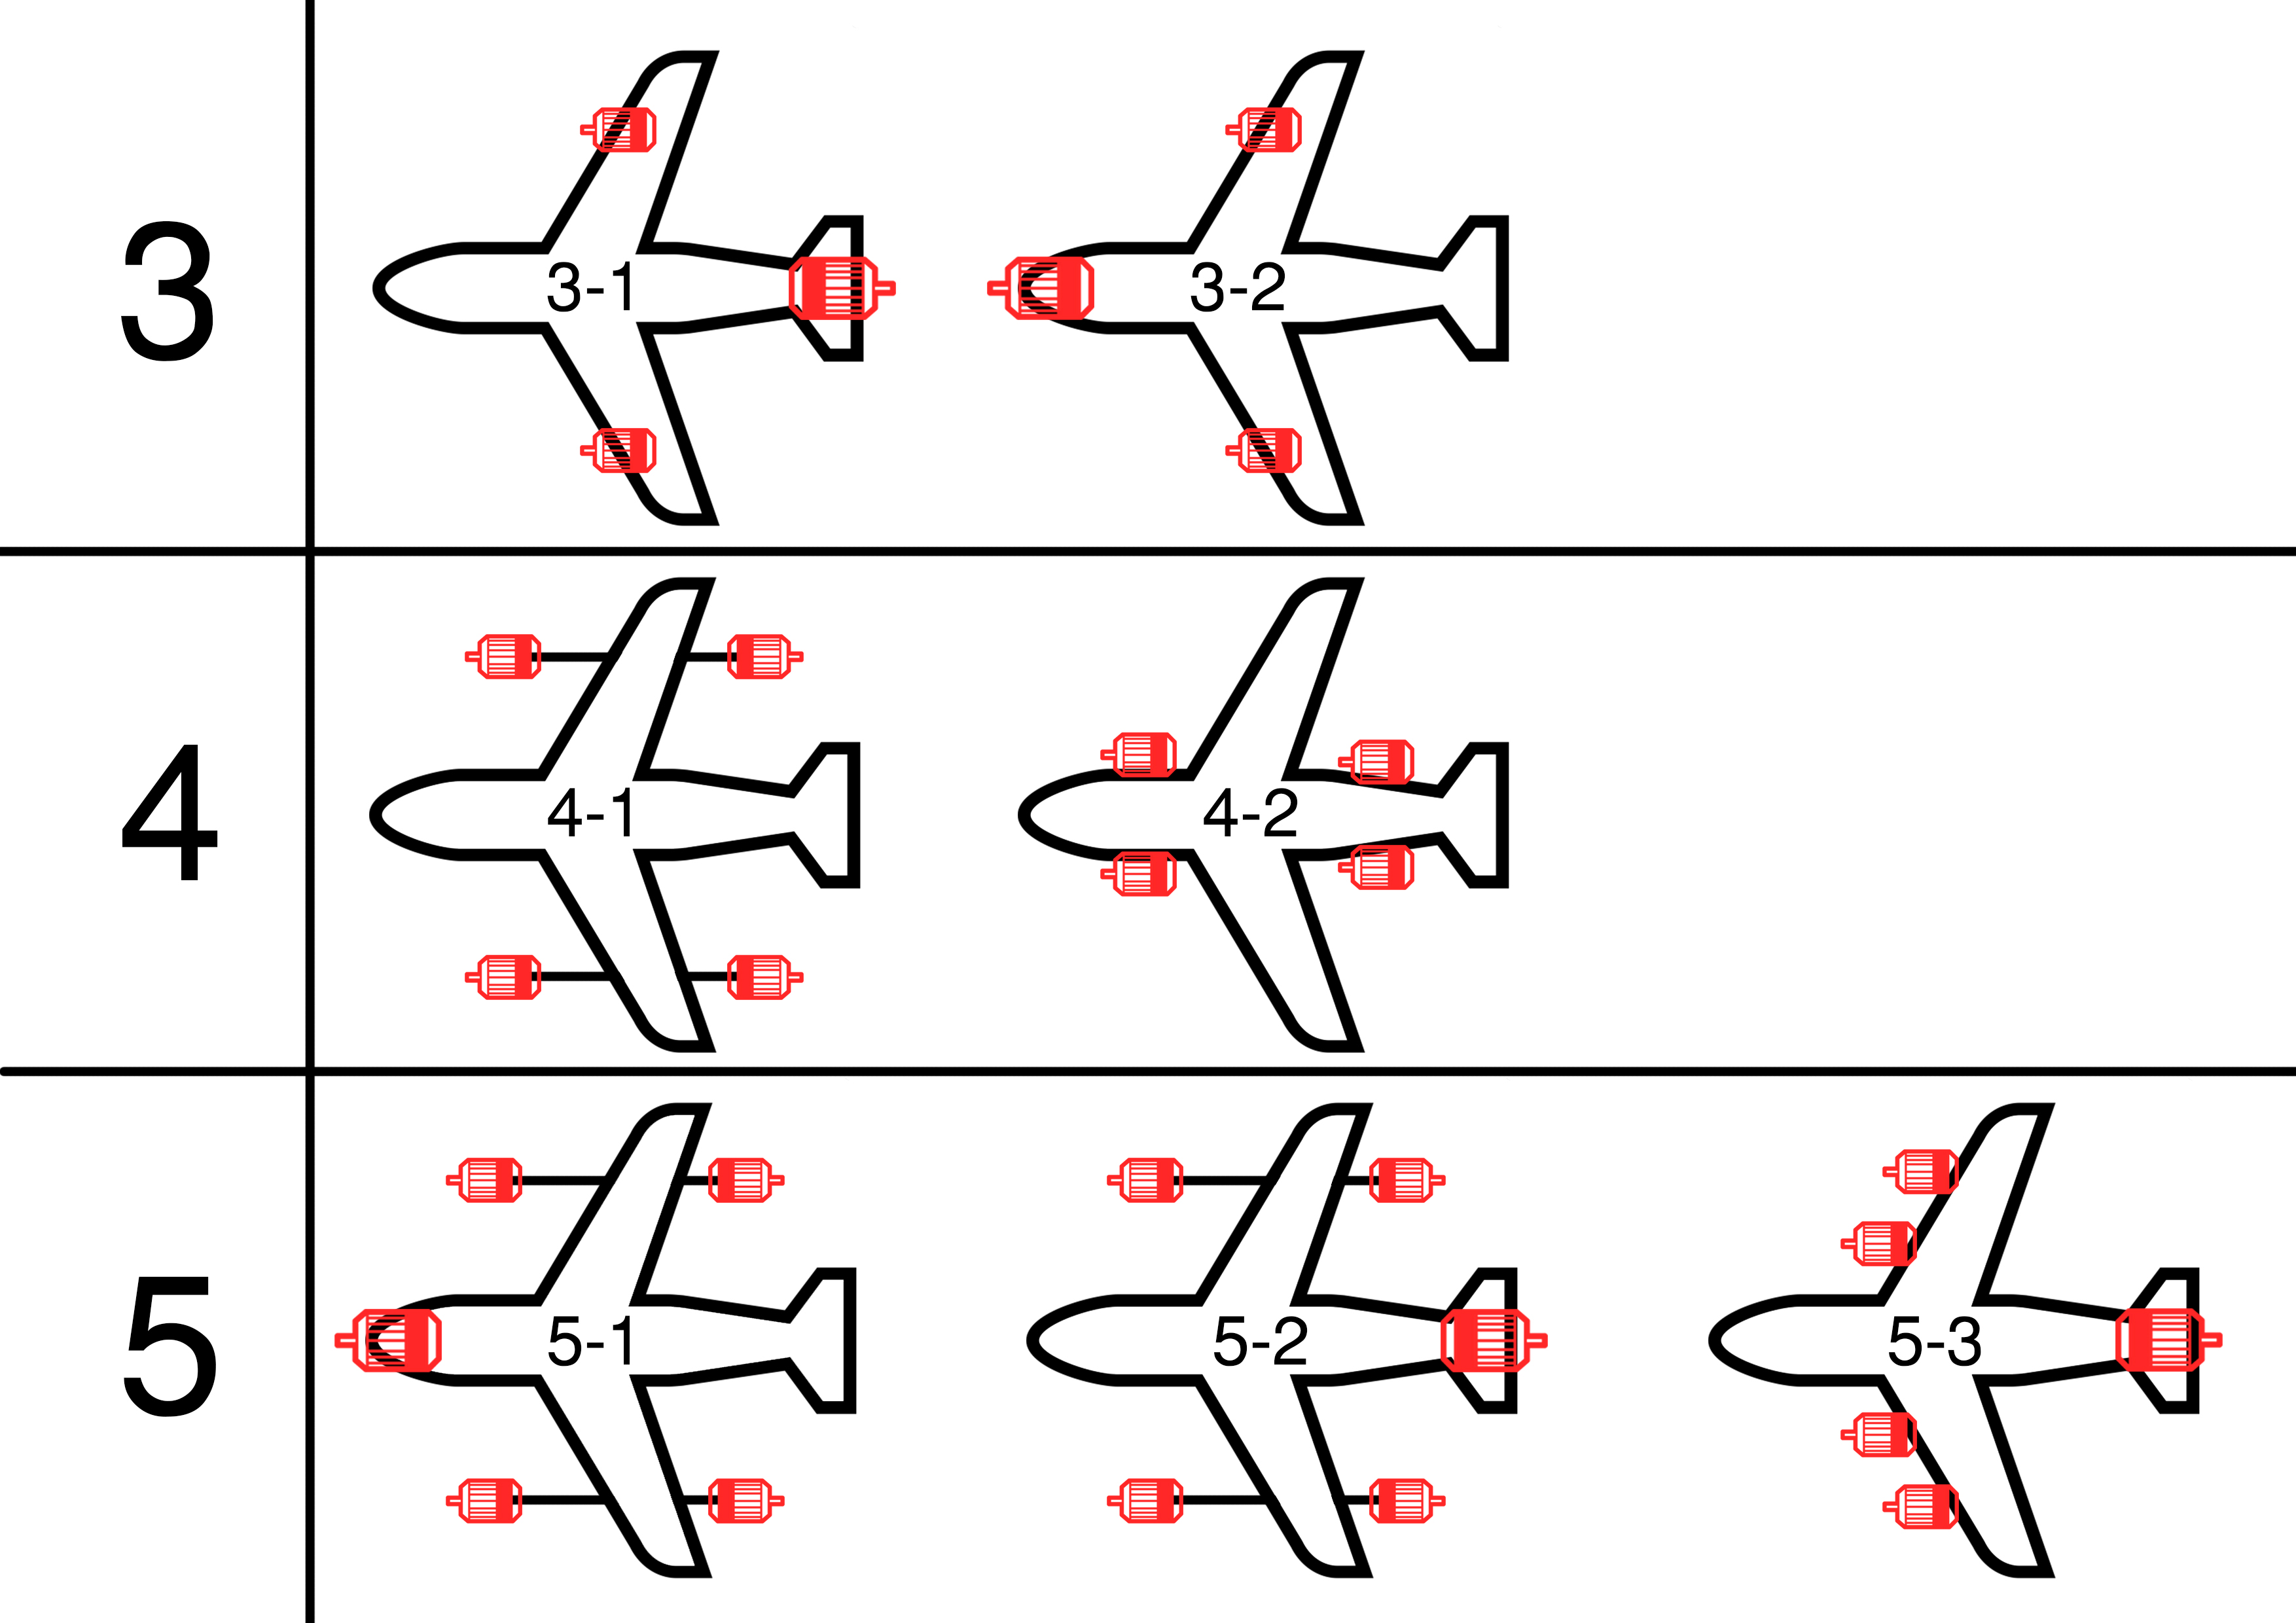
\includegraphics[width=0.8\textwidth]{PowerPropulsion/Figures/propconfig.jpg}
    \caption{Overview of Different Motor Configurations}
    \label{fig:motorconfig}
\end{figure}

\begin{itemize}
    \item \textbf{Three motors:} Consultation with the stability \& control department resulted in a conclusion that three-motor configurations (3-1 and 3-2) shall not be considered, since they do not generate sufficient controllability in VTOL operations.
    \item \textbf{Four motors:} Based on calculations, four-motor configurations turned out to be sufficient to meet both the required thrust and power output in VTOL and high-velocity cruise. Consultation with the stability \& control department resulted in a conclusion that a quadcopter setting (4-1) is advantageous over a body-mounted configuration (4-2), since a greater moment arm increases effectiveness of motors for VTOL stability.
    \item \textbf{Five motors:} Five-motor configurations (5-1, 5-2 and 5-3) were regarded as a solution to problems with propeller designing, however, the fifth motor solely dedicated for horizontal flight would allow the total cost and mass budget to easily exceed its limits.
\end{itemize}

\paragraph{Motor types:} There are two kinds of motors; brushed and brushless motors. Both types have advantages and disadvantages; brushed motors have for instance relative lower efficiency but are cheaper to produce than brushless motors. \autoref{tab:bbanal} shows a qualitative trade-off between the two type of motors. The superior option is indicated and the result is explained in the note column.

The major criteria are performance efficiency and cost. The capability to operate with high velocity is also important, since it is linked to the top-level performance requirement of max horizontal flight velocity of 200 km/h. Because there are also requirements related to noise emissions and required reliability, these aspects are also taken into account. Furthermore, due to the broad range of missions and operational conditions, the environmental resistance is also evaluated as a criterion.

\begin{table}[H]
    \centering
    \caption{Brushed vs. Brushless Motor Analysis}
    \label{tab:bbanal}
    \begin{tabular}{m{3cm}>{\centering}m{2cm}>{\centering}m{2cm}m{7cm}}
        \toprule        \textbf{}                                      & \centering\textbf{Brushed} & \centering\textbf{Brushless} & \textbf{Note}                                                                                                                                                                                                                           \\ \midrule
        \textbf{Efficiency}                            &                  & \cmark             & Brushed ranges from 75\% - 80\% in contrast to brushless, which ranges from 85\% - 90\%.\footnote{\url{https://quantumdevices.wordpress.com/2010/08/27/brushless-motors-vs-brush-motors-whats-the-difference/}, Accessed 20-06-2017} \\ \hdashline
        \textbf{Cost}                                  & \cmark           &                    & Brushed motors are typically lower in cost due to the simplicity and established production techniques \cite{wp}.                                                                                                                      \\\hdashline
        \textbf{Velocity}            &                  & \cmark             & Brushless motors typically generate higher angular velocity and torque, meaning it can operate with the higher-pitch propeller. The combination of a high pitch and RPM enable higher velocity for the brushless motor \cite{dae}.                       \\\hdashline
        \textbf{Reliability}                           &                  & \cmark             & Brushless motors have less parts that can potentially break or wear-out\footnote{\url{http://www.nmbtc.com/brushless-dc-motors/why-brushless-motors/}, Accessed 20-06-2017}.                                                               \\\hdashline
        \textbf{Environmental Resistance} & \cmark           &                    & Due to the simplicity of brushed motors, they can handle environmental conditions that are more hostile towards electronics and motor components \cite{dae}.                                                                                                  \\\hdashline
        \textbf{Noise Emission}                      &                  & \cmark             & Brushless motors emit less noise due to complete enclosure of internal components\footnote{\url{http://www.nmbtc.com/brushless-dc-motors/why-brushless-motors/}, Accessed 20-06-2017}.                                  \\ \bottomrule
    \end{tabular}
\end{table}
\nomenclature[A]{RPM}{Revolutions per minute}
\noindent A brushed motor has two main advantages, which are the lower cost and better environmental resistance. However, the rest of the criteria shows that the brushed motor performs worse than a brushless motor, especially in the performance-related criteria. The cost increase can be compensated by the budget and the environmental resistance can be drastically improved by the motor pylon. Thus, a brushless motor type is chosen for the Hybrid UAV design. Upon recommendation of ATMOS, the catalogue of Hacker-motors\footnote{\url{https://www.hacker-motor-shop.com/}, Accessed 19-06-2017} is chosen for getting necessary components.\\

\subsection{Utilised Tool Collection}
\paragraph{Static Thrust Calculator:}
The main tool used to find the right motor-propeller combination optimised for horizontal cruise flight is STC.\footnote{\url{http://www.godolloairport.hu/calc/strc_eng/index.htm}, Accessed 21-06-2017} The steps in the design approach in which this tool was utilised can be found in \autoref{sec:DAPNP}. The STC tool uses the propeller parameters (propeller pitch, diameter and type), RPM generated by the motor and the operational altitude as inputs. The provided thrust, required power and estimated operational speed is given as outputs. 

By using STC, required power and RPM output for a motor with a certain propeller diameter can be checked. Since there are more design parameters than constraints, an iterative process has to be initiated. Combinations of different propellers and motors with correct specifications have to be found. Using the Hacker-motors data set\cite{hackerdata}, an optimal motor-propeller combination is found.

\paragraph{Python Drag Calculator:}
To determine how much thrust the horizontal-flight optimised motor needs to produce, the drag in horizontal flight is computed. The PDC and \autoref{eq:d} are used. The equation is derived by replacing $C_{L}$ by the weight (W) divided by the dynamic pressure (q) and wing surface (S).\footnote{\url{http://nptel.ac.in/courses/101104007/Module2/Lec6.pdf}, Accessed 09-06-2017} As the drag calculation is complete, it is processed into the $P_{req}$ and required battery specifications.

%%bryan write here battery equations from drag calculator!!
%%i wrote it in under the Battery and Power Subsystem Components subsubsection

\begin{equation}
\label{eq:d}
    T_{req} = D = C_{D} q S = (C_{D_{0}} + \frac{C_{L}^{2}}{\pi AR e}) q S = C_{D_{0}}q S  + \frac{\frac{W^{2}}{q S}}{\pi AR e}
\end{equation}

The $P_{req}$ for maximum velocity operations is derived by multiplying the drag at maximum airspeed by that airspeed. The  $P_{req}$ can be found in \autoref{eq:p}.

\begin{equation}
\label{eq:p}
    P_{req} = D V = (C_{D_{0}} + \frac{C_{L}^{2}}{\pi AR e}) q S V =  \frac{1}{2} \rho V^{3} S C_{D_{0}} + \frac{\frac{W^{2}}{\frac{1}{2} \rho V S}}{\pi AR e}
\end{equation}

The values of the wing surface, aspect ratio, Oswald factor and $C_{D_{0}}$ are inputs provided by the aerodynamics department. The weight is taken from the mass budget and the corresponding requirement SYS-PH-2, which states that the maximum MTOW shall be 25kg.

\paragraph{Python VTOL Thrust Calculator:}
This tool computes the required thrust output in the VTOL mode as a function of the maximum power output of the motor and the propeller area. For the development of the tool, the conservation of momentum in helicopter climb/hover theory is used.\footnote{\url{http://s6.aeromech.usyd.edu.au/aerodynamics/index.php/sample-page/aircraft-performance/hoverclimbdescent-analysis/}, Accessed 19-06-2017} The equation for required thrust for hovering and climb is shown in \autoref{eq:hc}.

\begin{equation}
\label{eq:hc}
    T_{total,req} = (2 \rho A_{prop} P_{max}^{2})^{\frac{1}{3}}
\end{equation}

The required thrust value is provided by the stability \& control department by means of a moment equilibrium analysis. The maximum required thrust values are computed by analysing the moment with extreme c.g. position. For instance, with the most aft c.g. position, the aft motors have to provide significantly higher thrust levels. 

Furthermore, a margin has to be taken into account for the case a motor has to stabilise the UAV from incoming gust; during hovering, the thrust setting should not exceed 75\% to have some margin to correct disturbances.\\

\subsection{Propeller performance analysis:}

Within the motor-propeller design, several parameters have to be considered. To give an indication on the complexity of the cohesion of the parameters within the motor-propeller design process, an visual is shown in \autoref{fig:parap}. The black columns in the Figure are the two degrees of freedom, in the design process the propeller and motor with their corresponding parameters are selected. The difficulty however, is that the required output is in the form of the blue and red rows. It is the combination of parameters from both these two components that must meets the requirements. For instance, both the pitch (a propeller parameter) and the rotational speed (a motor parameter), determine whether of not the high-velocity requirement is met. So a right combination of motor-propeller is looked for. However, it is not just the high-velocity requirements. Also the thrust output, which is depending on both the propeller diameter and the motor power output, is a requirement where the motor-propeller selection should be optimised for. The two requirements both pose constrains on the selection process, but are also conflicting one another; optimising for requirement one, might be a very inefficient or even infeasible combination for requirement two. The difficulty is to find a motor-propeller selection that meets both the requirements in the optimal way.

\begin{figure}[H]
    \centering
    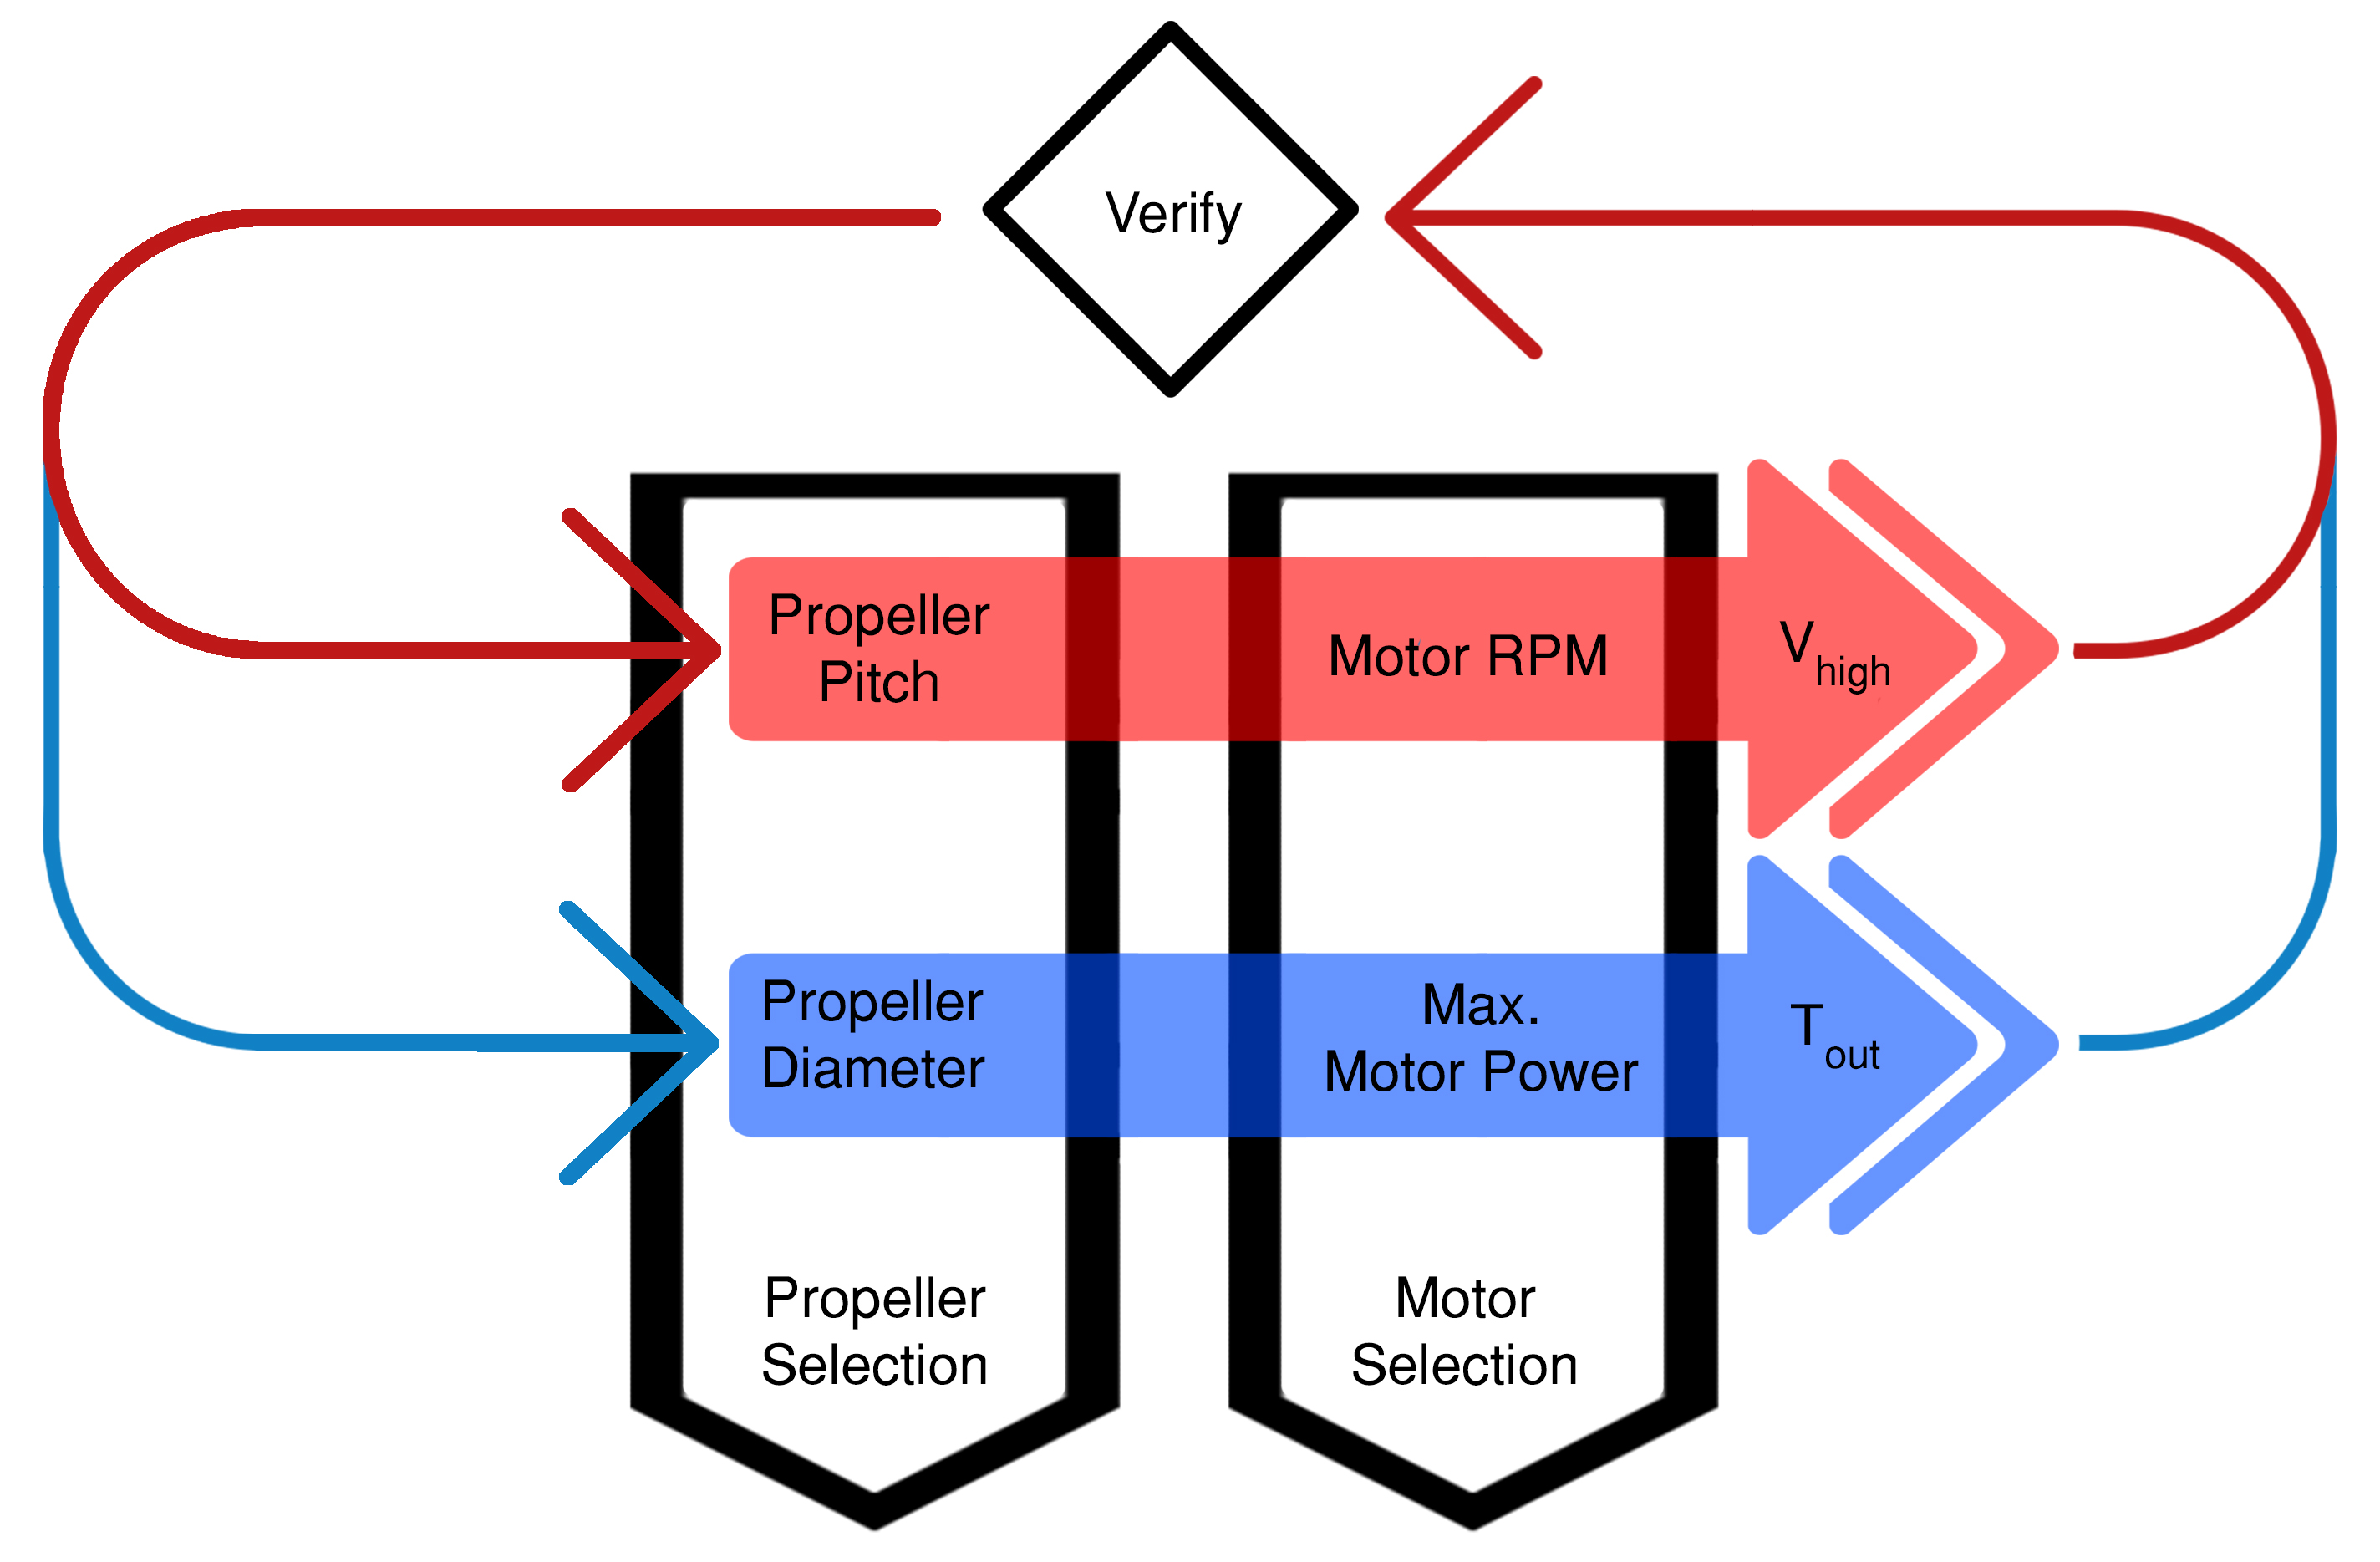
\includegraphics[width=0.87\textwidth]{PowerPropulsion/Figures/propnpowerrocessor.jpg}
    \caption{Parameter Relationship within Motor-propeller Design}
    \label{fig:parap}
\end{figure}

The optimal motor-propeller selection is done by means of an iterative process. For different propeller and motor choice, the requirements are verified and fed back into the system. In this way, the design converges to the propeller and motor selection that is optimal for both performance requirements.  

The performance of a propeller is very sensitive to operational conditions; propellers are designed for specific conditions such as flight speed and RPM inputs. As seen in \autoref{sec:DAPNP}, the first step in the design approach is related to the propeller design. The propeller design, especially the pitch, is highly significant to the operational airspeed at which the UAV can operate.



\begin{figure}[H]
    \centering
    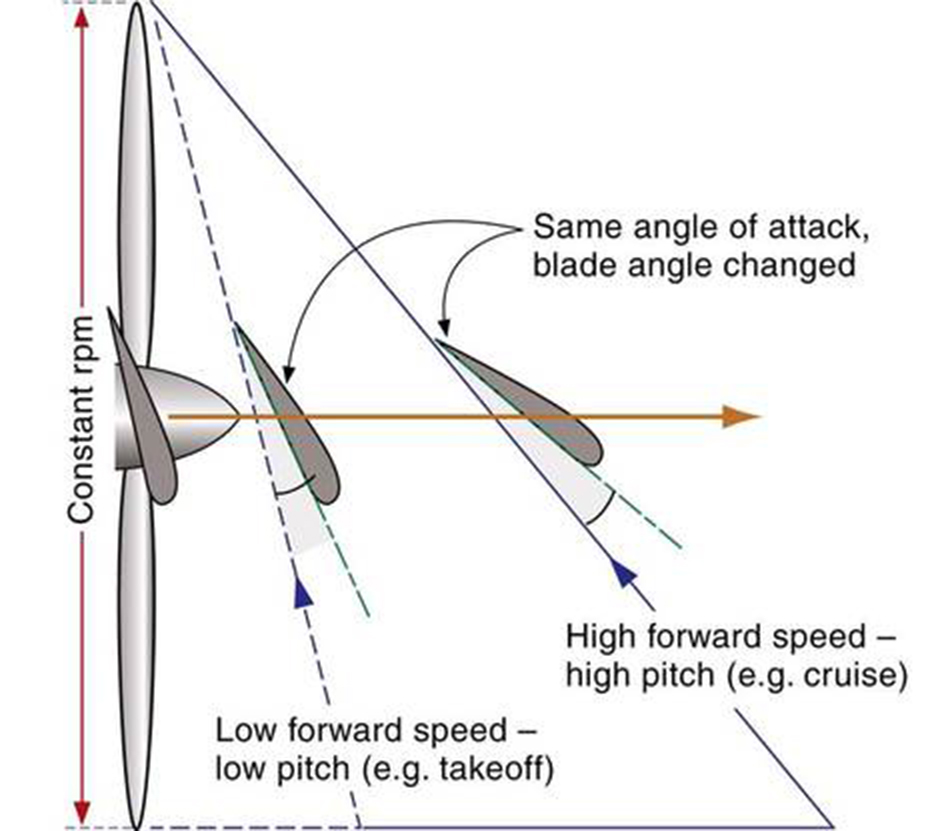
\includegraphics[width=0.45\textwidth]{PowerPropulsion/Figures/proppitch.jpg}
    \caption{Theoretical Relation between Propeller Pitch and Flight Velocity\footnote{\url{http://www.pilotwings.org/propellers.html}, Accessed 21-06-2017}}
    \label{fig:pitch}
\end{figure}


A propeller is essentially a wing in rotating motion and acts as a regular wing, as a propeller also experiences stalling phenomena in certain flight conditions. In case a propeller pitch is high, the desired airspeed is also high; a high-pitched propeller has an increased risk of stalling àt low airspeed. \autoref{fig:pitch} shows that a propeller with higher pitch will have an equal angle of attack as a lower pitched propeller if the flight velocity is higher. 

Within the specifications list of a propeller, the pitch is often indicated in inches and not as an angle. The inch value is the distance that the propeller would travel during one revolution. It means that the pitch together with the RPM with which it rotates determines the cruise velocity, as indicated in \autoref{eq:RPM}.

\nomenclature[A]{RPM}{Revolution Per Minute}

\begin{equation}
\label{eq:RPM}
    V_{cruise} = \textrm{Pitch} \cdot \frac{RPM}{60}
\end{equation}

This shows that different pitched propellers (given a constant RPM) have own `referred operational regime'. It means that the different operational phases should be addressed and analysed for the design. In this UAV design, the two critical flight phases are VTOL and high-velocity horizontal flight. 
\begin{enumerate}
    \item In case of the VTOL phase, the flow velocity is relatively low and the required thrust is high. The propeller that is optimised for VTOL will have a low pitch and a large diameter.
    \item In case of high-velocity horizontal flight, lower thrust is required, but the flight velocities are significantly higher. This will result in a significantly higher required propeller pitch, with a low desired propeller diameter.
\end{enumerate}

%%%%%%%%%%% stopped here, due to lack of time - Bryan @1530 23/06
%%%%%%%%%%% resuming @1756 23/06

Since propellers only perform optimally in their specific operational regime, there is a problem to perform hybrid operations with the same propellers; propellers optimised for VTOL will perform poorly in horizontal flight and vice versa. Several solutions are considered to optimise the propulsion system both for VTOL and horizontal flight. By means of brainstorming and consulting experts in the field of propeller design, the following solutions are found to be worthy for further analysis.\\

\noindent \textbf{Solution 1} Use four propellers purely for the VTOL operation and install a fifth motor as either a pusher or a puller configuration to sustain the horizontal cruise flight. 

This solution is proven to be infeasible with respect to both the mass and cost budget; a fifth horizontal flight motor is too heavy and will increase the total cost to an undesirable extent. Also, not using four of the five motors during horizontal flight is regarded as highly inefficient; the VTOL phase is just a small fraction of the mission scenarios, and the four propellers will simply be inducing extra drag during the rest of the missions.\\

\noindent \textbf{Solution 2} Equip all four motors with double propeller; one optimised for VTOL and the other for horizontal flight. During VTOL operations, the horizontal propellers are retracted, and the VTOL propellers are retracted during horizontal flight.

The double propeller solution is not feasible as well, since the concept is still in the experimental phase. Double propellers introduce great complexity to the system; the rotating of an extra pair of propellers may cause difficulties in balancing the rotors. Furthermore, this foldable propeller system also increases the drag. For these reasons, this solution is regarded as infeasible.\\

\noindent \textbf{Solution 3} Implement four similar propellers that are not optimised for specific operations; this means implement a kind of propeller that has both in VTOL and horizontal flight a moderate performance. To see the feasibility of this solution, further analysis is required. First the 200 km/h cruise flight has to be ensured, which means, according to \autoref{eq:RPM} choosing a motor-propeller configuration with sufficient pitch and RPM output. Next to that, the propeller should have sufficient diameter to generate enough thrust for VTOL operations.

For the horizontal high-velocity flight performance analysis the STC tool used. For the VTOL performance, the VTOL Thrust Calculator was utilised. By trial and error, there was concluded that there exist no motor that could provide enough power to operate a sufficiently pitched big diameter propeller at high RPM\footnote{Motors from the Hackers-motor data set\footnote{Motors from the Hackers-motor data set}. If such a motor would exist, it would for sure exceed the cost and mass budget. Furthermore, if both the front and aft propellers operate at the same time in horizontal flight, another undesirable phenomena will occur; since the propellers are longitudinally aligned, a propeller wash is created by the front propellers affecting the aft propellers by decreasing their efficiency \cite{wash}.\\ 

\noindent \textbf{Solution 4} Using only one pair of propellers for horizontal flight, and providing the other pair of propellers with folding/feathering capability. The advantage of this solution is that there is no wash of the front propeller that influences the aft propeller, since the front propeller is folded in horizontal flight. The downside of this solution is that during VTOL, the front propellers have to compensate for the poor performing aft propellers; the aft are after all optimised for horizontal flight. This means that the front motor-propeller combination has to be optimised for VTOL and needs to provide a significant thrust output. This solution needs  further analysis to see if motor-propeller combinations can be found that fit in the cost and mass budget and still meet the performance requirements; this is done in the next paragraph. %JUSTIFY PUSHER PROP CHOICE. CHECK THE WRITTEN TEXT AND SEE IF IT'S GOOD

%A thing that can already be constraint is the fact that in horizontal flight only the aft motors and not the front motors

% why that diameter???
\nomenclature[B]{$T_{req}$}{Thrust required}
\nomenclature[B]{$T_{max,out}$}{Maximum thrust output}
\nomenclature[B]{$T_{reduced,out}$}{Maximum thrust output without overheating}


\subsection{Propeller and Corresponding Motor Selection}
First of all the required pitch was determined; after consulting experts, the highest propeller pitch on the market was found to be approximately 14 inch. To prevent the difficulty of coming up with a custom designed propeller, the choice was made to go with a conventional design; a propeller of 14 inch pitch with 11 inch diameter was chosen (11x14). By rewriting \autoref{eq:RPM} and transforming the units to the metric system, a required rotational speed of 9380 RPM was obtained. The motor that comes closest to this requirement is the A50-12L, which has a maximum rotational speed of 9429 RPM\footnote{\url{https://www.hacker-motor-shop.com/Brushless-Motors/Glider-drives/Glider-10kg/A50-12-L-V4.htm?shop=hacker_e&SessionId=&a=article&ProdNr=15726840&p=7202}, Accessed 22-06-2017}. 

\begin{equation*}
RPM = \frac{V_{cruise}}{\textrm{Pitch}} \cdot 60 = \frac{55.6}{14 \cdot 0.0254} \cdot 60  = 9380  \textrm{RPM}
\end{equation*}


\begin{comment}
\autoref{table:A50} gives the main specifications of this selected aft motor.

\begin{table}[]
\centering
\caption{Main specifications A50-12L V4 motor}
\label{table:A50}
\begin{tabular}{ll}
\hline
\multicolumn{2}{l}{A50-12L V4} \\ \hline
Amps               & 66        \\
Power       & 2009 [W]     \\
RPM                & 9429      \\ \hline
\end{tabular}
\end{table}
\end{comment}

The next step was to verify that the motor specifications met the required values; this was done for first for vertical operations and secondly for horizontal flight.\\

\noindent \textbf{Vertical performance analysis aft motor unit} For the vertical performance, the maximum power output of the selected A50-12L motor was used for the thrust calculation. As a side note, the motor can only provide the maximum power for a limited time; after a certain time it might overheat. However, even if a reduced maximum power is taken to be 5\% less than the actual value, the thrust output is still sufficient since it only decreases to a value of 80.4 N. \autoref{tab:vert_perf_anal} shows that the A50-12L motor can easily provide the 71.9 N of required thrust.

\begin{table}[H]
\centering
\caption{Vertical Performance Analysis of A50-12L V4 Motor}
\label{tab:vert_perf_anal}
    \begin{tabular}{lcl}
    \toprule
                 &\bfseries Value & \bfseries Used Tool                     \\ \midrule
    $T_{req}$ {[}N{]} & 71.9  & Moment equilibrium            \\\hdashline
    $T_{max,out}$ {[}N{]} & 84.6  & Python VTOL Thrust Calculator           \\\hdashline
    $T_{reduced,out}$ {[}N{]} & 80.4  & Python VTOL Thrust Calculator \\ \bottomrule
    \end{tabular}
\end{table}

\noindent \textbf{Horizontal performance analysis aft motor unit}
In horizontal maximum velocity cruise flight the required thrust, which equals the drag, was calculated using the Python Drag Calculator. This turned out to be a total of 12.42 N per motor. The thrust provided by the motor-propeller combination was computed by the STC; that turned out to be approximately 4.5 N more per motor, clearly sufficient to compensate for the drag. Also the power required for the most critical operational phase (maximum velocity flight), that was computed by the Python Drag Calculator, turned out to be lower as the maximum power output of the selected motor. The result shown in \autoref{tab:hor}, show as well that the A50-12L V4 is an optimal choice.

\begin{table}[H]
\centering
\caption{Horizontal Performance Analysis of the A50-12L V4 Motor}
\label{tab:hor}
    \begin{tabular}{lcl}
    \toprule
                              &\bfseries Value  &\bfseries Used Tool                     \\ \midrule
    $T_{req,max}$  {[}N{]}         & 12.42  & Python Drag Calculator        \\\hdashline
    $T_{out,max}$ {[}N{]}              & 16.97  & Static Thrust Calculator \\\hdashline
    $P_{req}$ (Max. speed) {[}W{]}  & 1381 & Python Drag Calculator        \\\hdashline
    $P_{req}$ (Max. range) {[}W{]}       & 314.2  & Python Drag Calculator        \\\hdashline
    $P_{req}$ (Max. endurance) {[}W{]}  & 260    & Python Drag Calculator        \\\hdashline
    $P_{out,max}${[}W{]}            & 2009   & Given specification 
        \\\bottomrule
    \end{tabular}
\end{table}
\nomenclature[B]{$P_{req}$}{Power required \nomunit{W}}
\nomenclature[B]{$T_{req,max}$}{Maximum required thrust \nomunit{N}}
\nomenclature[B]{$T_{out,max}$}{Maximum thrust output needed \nomunit{N}}
\nomenclature[B]{$P_{out,max}$}{Power required \nomunit{W}}

\noindent \textbf{Vertical performance analysis front motor unit:}
Finally, the front motor-propeller combination has to be chosen, this motor is optimised for VTOL. This means it only performs vertical operations; no horizontal flight, since then the front propellers are in folded or feathering mode.

After some iterations, the chosen selection is the Q60-7M F3A motor.

\begin{table}[H]
\centering
\caption{Vertical Performance Analysis of Q60-7M Motor}
\label{tab:vert_Q60-7M}
    \begin{tabular}{lcl}
    \toprule
                 &\bfseries Value &\bfseries Used Tool                     \\ \midrule
    $T_{req}$ {[}N{]} & 124.0  & Moment equilibrium            \\\hdashline
    $T_{max,out}$ {[}N{]} & 135.57  & Python VTOL Thrust Calculator           \\\hdashline
    $T_{reduced,out}$ {[}N{]} & 81.5  & Python VTOL Thrust Calculator \\ \bottomrule
    \end{tabular}
\end{table}


Although \autoref{sec:MP} shows only the analysis of one motor-propeller combination, several combinations were analysed; after all the entire approach was iterative. The A50-12L V4 motor with a 11x14 propeller proved to be optimal, that is why only the analysis of this engine unit is treated.

\begin{comment}
\textbf{Conclusion: }
In results!

The front propeller will be optimised for VTOL. This means that the pitch is nominal and the diameter is as big as possible. The diameter, however, is constrained by the geometry of the pylons; it is undesirable for the propeller to cover the wings, since that would influence the propeller performance in a negative way. That means that overlap of the propeller with the wing is aimed to be as small as possible.


How to do hybrid operations:
By optimising the front ones for VTOL and make them the main VTOL contributors, the aft motors are optimised for horizontal operations. In this way they can assist partly in the VTOL phase and serve as main contributor to the horizontal flight phase. 
\end{comment}


\subsection{Battery and Power Subsystem Components}

Required power can be found using \autoref{eq:p}. Velocity for each extreme flight scenario is defined based on the performance analysis in the previous phase of the project.\cite{midterm} Important parameters such as wing surface area, aspect ratio, Oswald factor and zero-lift drag coefficient are redetermined and used for the velocity calculation. The required power is divided by voltage to obtain current. With the determined current, \autoref{eq:battcap} is used to calculate the required battery capacity for each extreme flight scenario, which can be seen in \autoref{tab:extreme}. It can be seen that the max.range flight scenario requires the highest battery capacity of 16100 [mAh]. The duration of the max.speed flight is defined to be 15 minutes, as longer max.speed flight puts heavy loads on motors and battery packs.
\nomenclature[B]{$C_{req}$}{Required battery capacity \nomunit{mAh}}
\nomenclature[B]{I}{Current \nomunit{A}}
\nomenclature[B]{D}{Drag \nomunit{N}}
\nomenclature[B]{$C_{req,efs}$}{Required battery capacity for extreme flight scenario \nomunit{mAh}}


\begin{equation}
\label{eq:battcap}
   C_{req} = I*\frac{t_{flight}}{60}*1000
\end{equation}

\begin{table}[H]
\centering
\caption{Battery Capactiy for Extreme Flight Scenarios}
\label{tab:extreme}
    \begin{tabular}{m{3.2cm}>{\centering}m{1.5cm}>{\centering}m{2cm}>{\centering}m{1.3cm}>{\centering}m{1.5cm}c}
    \toprule
    \bfseries Flight Scenario  &\bfseries  V [m/s] &\bfseries  $t_{flight}$ [min] &\bfseries  D [N] & \bfseries $P_{req}$ [W] & \bfseries $C_{req,efs}$ [mAh] \\\midrule
    Max.speed     & 55.6    & 15             & 24.4  & 1360      & 9180        \\\hdashline
    Max.range     & 29      & 115            & 10.7  & 311       & \textbf{16100}       \\\hdashline
    Max.endurance & 24      & 60             & 10.8  & 258       & 6980        \\\bottomrule
    \end{tabular}
\end{table}

\nomenclature[B]{$V$}{Airspeed \nomunit{m/s}}
\nomenclature[B]{$t_{flight}$}{Flight duration \nomunit{min}}
\nomenclature[B]{$P_{req}$}{Required power \nomunit{W}}


The essential flight phases are defined by requirements SYS-PF-2.3 and SYS-PF-2.4. Thus, the duration for hovering is 5 minutes while the duration for VTOL is 1 minute. In order to compute required power for VTOL and hovering, \autoref{eq:hc} can be rewritten in terms of power as following:

\begin{equation}
\label{eq:hc2}
    P_{req} = \sqrt{\frac{T_{req}^3}{2*\rho*A_{prop}}}
\end{equation}

\nomenclature[B]{$A_{prop}$}{Propeller area}

\autoref{eq:hc2} is used to compute required power for front and aft motors during VTOL and hovering, which can be seen in \autoref{tab:essential}. The required battery capacity is 8090 [mAh], by summing $C_{req,efp}$ for VTOL and hovering.

\begin{table}[H]
\centering
\caption{Battery Capacity for Essential Flight Phases}
\label{tab:essential}
    \begin{tabular}{m{2cm}ccccc}
    \toprule
             &\bfseries $t_{flight}$ [min] &\bfseries $P_{req,front}$ [W] &\bfseries $P_{req,aft}$ [W] &\bfseries Sum [W]      &\bfseries $C_{req,efp}$ [mAh] \\\midrule
    VTOL     & 1              & 1660            & 955           & 2*(1660+955) & \textbf{2360}            \\\hdashline
    Hovering & 5              & 600             & 672           & 2*(600+672)  & \textbf{5730}  \\\bottomrule         
    \end{tabular}
\end{table}

\nomenclature[B]{$P_{req,front}$}{Required power for a front motor \nomunit{W}}
\nomenclature[B]{$P_{req,aft}$}{Required power for an aft motor \nomunit{W}}
\nomenclature[B]{$C_{req,efp}$}{Required battery capacity for essential flight phases \nomunit{mAh}}

Power usage of other subsystems must be considered to determine the final battery sizing. Based on an estimation by the command \& data handling department, the power usage of avionics is 9.23 [W]. Since this value is extremely small compared to required power for max.range flight scenario (9.23 vs. 16100), the power usage of avionics is assumed to be negligible. Then, the final required battery capacity is determined to be 16100 + 8090 = 24190 [mAh]. Since the front motors are 10S, a battery pack with 10S should be used. Aft motors are 8S, but a DC/DC converter will be installed in order to downscale the voltage. It seems that there are very few 10S battery packs with high capacity. `ZIPPY Compact 5800 mAh 10S 25C Lipo Pack' is selected, as it provides sufficient current and capacity for the propulsion subsystem. 5 battery packs will be used, from 24190 [mAh]/5800 [mAh] = 4.17.\\

As the battery is chosen, battery cable and connectors for the cable must be selected. `Turnigy High Quality 8AWG Silicone Wire 1m' and `Nylon XT90 Connectors Male/Female' are selected for battery cable and connectors. The cable is estimated to be around 4 meters based on the layout of the UAV. %refer to a layout? right now there is nothing

The cost and mass budget has to be reviewed to see if chosen power subsystem components are within the budgets. According to \autoref{tab:massbudget}, the mass budget and cost budget for the power subsystem is 7.6 kg and 950 EUR respectively, including 5\% contingency. \autoref{tab:tmcpsc} shows that the actual mass and cost of the power subsystem is 6.9 kg and 694.73 EUR respectively. Thus, the chosen components are within the budgets.

\begin{table}[H]
\centering
\caption{Total Mass and Cost of Power Subsystem Components}
\label{tab:tmcpsc}
    \begin{tabular}{lcc}
    \toprule
    \bfseries Power components   &\bfseries  Total mass [kg] &\bfseries Total cost [\euro] \\\midrule
    Battery packs      & 6.34            & 673                \\\hdashline
    Battery cables     & 0.48            & 13.3               \\\hdashline
    Battery connectors & 0.078           & 8.43               \\\hdashline
    Sum                & \textbf{6.90}            & \textbf{694.73}        \\\bottomrule       
    \end{tabular}
\end{table}

\paragraph{Payload range diagram} For certain ranges, part of the payload capacity has to be sacrificed to be exchanged with additional battery. To show the payload capacity for different ranges, a payload range diagram is shown in \autoref{fig:PRD}.

\begin{figure}[H]
    \centering
    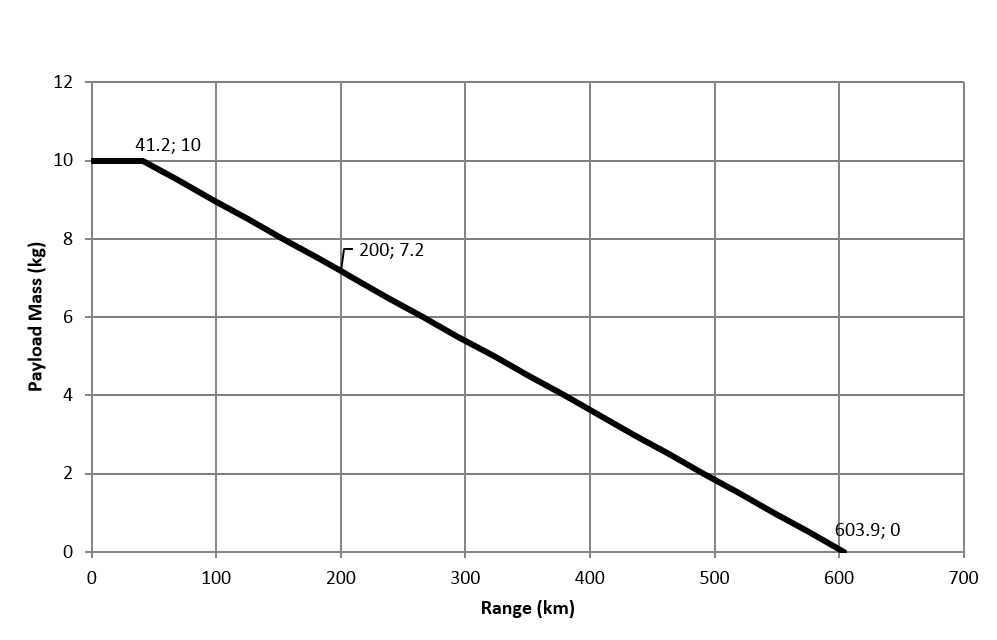
\includegraphics[width=0.87\textwidth]{PowerPropulsion/Figures/PRDiagram.png}
    \caption{Payload Range Diagram}
    \label{fig:PRD}
\end{figure}

The equation for the range is found by dividing the battery, which is obtained by multiplying the battery mass by the specific capacity, by the battery capacity required for 200km range. This gives a $C_{bat}/C_{200km}$ - ratio. Furthermore, due to the assumption that the power output during operation is approximately constant, the capacity is assumed linearly related with range. This enables the range to be calculated by multiplying the capacity ratio by 200km, as shown in \autoref{eq:PRD}

\begin{equation}
\label{eq:PRD}
    R = \frac{C_{bat}}{C_{200km}} \cdot 200  =\frac{M_{bat} \cdot \frac{C}{M}}{C_{200km}} \cdot 200 
\end{equation}

There are a number of conclusions that can be drawn form the \autoref{eq:PRD}. First of all, the curve shows first a horizontal line segment, after which it at a certain range starts descending in a linear way with a slope of 56 km/kg. With a maximum payload capacity of 10kg, the UAV has a range up to a 41.2km. For top level range requirement SYS-PF-1.3R, the corresponding payload capacity for a maximum range of 200km will be 7.2kg. The absolute maximum range, which can be covered if all payload capacity is used for additional battery, is 603.9km. 


%3) Power:
%- Battery that sustain the motors (VTOL, high-speed) and all the other subsystem (Look into the C-rating, discharge value.);
%- Cable harness (layout, mass estimation, regard accessibility and Assembly capabilities);
%- Electrical component and circuits design.

\subsection{Rotating Mechanism Components}
A simple rotating mechanism with fiberglass reinforced nylon parts and a servo is chosen, as very few off-the-shelf rotating mechanism components exist. After a market research, a tilt mechanism for a tricopter is considered, although it may require minor modifications to be retrofitted to the Hybrid UAV. A specific servo is recommended along with the mechanism, as they are designed to be used as a set. The quantity, mass and cost of rotating mechanism components can be seen in \autoref{tab:PNPresults}.

\subsection{Conclusion; Component Selection and Recommendations}
All the chosen components for power \& propulsion subsystems can be seen in \autoref{tab:PNPresults}. Besides all the product names, it also shows the unit mass and cost, based on this there can be concluded whether or not the selection meets the budget constraint.
\begin{table}[H]
\centering
\caption{Off-the-shelf Component Choice Power \& Propulsion Subsystems}
\label{tab:PNPresults}
    \begin{tabular}{m{4cm}m{4cm}m{0.6cm}cc}
    \toprule
    \bfseries Component                   &\bfseries Product Name                                                     &\bfseries Q. &\bfseries Unit Mass {[g]} &\bfseries Unit Cost{[\euro]} \\ \midrule
    Front Motor        & Hacker Q60-7M (10S)                                                             & 2           & 520                        & 410                      \\\hdashline
    Front Propeller    & AC Carbon 16x10                                                           & 2           & 25                         & 11.8                      \\\hdashline
    Front Speed Controller & MasterSPIN 99 Pro                                                         & 2           & 105                        & 229                      \\\hdashline
    Front spinner     & Spinner RFM 40x6                                                            & 2  & n.a & 30.9
                      \\\hdashline
    Aft Motor          & Hacker A50-12L (8S)                                                           & 2           & 445                        & 184                      \\\hdashline
    Aft Propeller      & APC 11x14                                                                 & 2           & 40                         & 3.50                       \\\hdashline
    Aft Speed Controller   & X-70-SB                                                                   & 2           & 54                         & 99                       \\\hdashline
    Aft spinner        & Ae-spinner A/K 45                                                      &  2        & n.a & 8.65
                    \\\hdashline
    DC - DC Converter    & LM2596 DC 3.2-40V to 1.25-37V                                    & 2    & n.a             & 2.70                        \\\hdashline
    Rotating Mechanism     & Tricopter Tilt Mechanism                                            & 4           & 10.6                       & 8.50                       \\\hdashline
    Servo              & BMS-210DMH                                                               & 4           & 17.5                        & 24.2                      \\\hdashline
    Servo wire        & DITEX Servowire Extension                                              &  4          &  n.a  & 7.30
                    \\\hdashline
    Battery            & Zippy Compact 5800mAh 10S Lipo                                           & 5           & 1268                       & 134.5
    \\\hdashline
    Power cabling            & Turnigy HQ 8 AWG Silicon wire                                             & 4           & 120/m                     & 3.50/m                 \\ \hline \hdashline
     \textbf{Total}   &     &    &  9310.4 & 
        \\\bottomrule
    \end{tabular}
\end{table}



\begin{comment}
Recommandations???

4) Optional: look into other propulsion types (break with electric prop. requirement):
- Electric VS. Combustion
- Electric VS. Hybrid propulsion

Do a more accurate research in propeller efficiency

recom: look into propeller detail in more detail

Test motor-propeller efficiency by an experimental setup; theoretical efficiencies are often not accurate. 

\end{comment}


\section{Verification \& Validation}
\label{sec:VNVPNP}

In order to ensure accuracy the power \& propulsion analysis, the methods used to perform the analysis have to be verified, and the corresponding results as well as tools used have to be validated.
\subsection{Verification}
Inputs used for PDC have to be checked. The input parameters of PDC that are dependent on other departments are as following: weight, air density, zero-lift drag coefficient, wing surface area, aspect ratio, Oswald factor. In the beginning of the iteration process, the parameters were approximated from the previous phase of the project and used. Initial calculations were carried out components were chosen based on the calculations. Since the parameters directly come from the aerodynamics department, inter-communications between the power \& propulsion department  and aerodynamics department were established and finalised values are used for the final power \& propulsion subsystem design. Thus, the parameters used in PDC are up to date and correct.

\subsection{Validation}
\subsubsection*{Tool Validation}
Python is primarily used to generate models for the analysis. It is assumed that Python is validated by a group of experts in various industries.

\subsubsection*{Model Validation}
STC contain models for the analysis. Since STC itself does not provide any codes, the validation of STC is done with a method of analysis. In order to check if the model of STC is correct, a set of real life data is used as an input for the method of analysis. Five arbitrary motor and propeller combinations are used to validate the model, which can be seen in \autoref{tab:stcvali}. Input parameters for the validation are propeller diameter \& pitch, RPM and propeller type. The output parameter is power. The STC power values have difference of less than 5 \% with respect to the reference power value from the Hacker-motor data sheet.\cite{hackerdata} Thus, values generated by STC are assumed to be valid and the model is validated.

\begin{table}[H]
\centering
\caption{STC Validation}
\label{tab:stcvali}
    \begin{tabular}{lccc}
    \toprule
             &\bfseries Reference power value [W] &\bfseries STC power value [W] &\bfseries Difference [\%] \\\midrule
    A50-16S  & 1117                      & 1127                & 0.887          \\\hdashline
    A40-10L  & 945                       & 909                 & 3.96           \\\hdashline
    C50-13XL & 2592                      & 2611                & 0.728          \\\hdashline
    A200-8   & 8820                      & 8741                & 0.904          \\\hdashline
    Q80-11S  & 3038                      & 2908                & 4.47     \\\bottomrule     
    \end{tabular}
\end{table}
